\documentclass[10pt]{article}
\usepackage{fancyhdr, geometry, graphicx, tikz}
\usepackage{mathpartir}
%\usetikzlibrary{positioning}
\usepackage{amssymb, amsmath}
\usepackage{enumerate, verbatim}
%\graphicspath{ {.} }
\pagestyle{fancy}

\lhead{\sf CS 6110 Homework 1}
\rhead{\sf Giang Nguyen (htn26) and Quinn Beightol (qeb2)}

\newcommand{\steps}{\longrightarrow}
\newcommand{\apply}{\lambda x. \lambda y. x~y}

\newcommand{\Rule}[3]{
  [\textsc{#1}]~
  \label{rule:#1}
  \hfill
  \ensuremath{\inferrule{#2}{#3}}
  \hfill
}


\begin{document}
\subsection*{\sf 1 Free and Bound Variables}
%\begin{graveyard}
  % $$
  % % \lambda a. \left (
  % %   \lambda b. \left (
  % %     \lambda c. \left (
  % %      \left( \left ( \left ((a a) (\lambda b. b) \right ) b \right ) c \right ) c
  % %     \right )
  % %   \right )
  % % \right )
  % \left ( (a~a)~(\lambda b. b) \right )
  % $$
  % \begin{center} \begin{tikzpicture}[node distance=0.5cm]
  %   \node (absA) {$\lambda a.$};
  %   \node (absB1) [right=of absA] {$\lambda b.$};
  %   \node (absC) [right=of absB1] {$\lambda c.$};
  %   \node[rectangle, draw] (a1)    [right=of absC] {$a$};
  %   \node[rectangle, draw] (a2)   [right=of a1] {$a$};
  %   \node (absB2) [right=of a2] {$\lambda b.$};
  %   \node[rectangle, draw] (b1) [right=of absB2] {$b$};
  %   \node[rectangle, draw] (b2) [right= of b1] {$b$};
  %   \node[rectangle, draw] (c1) [right=of b2]{$c$};
  %   \node[rectangle, draw] (c2) [right=of c1]{$c$};
  %   \path[->]
  %     (a1) edge [bend right]  node {} (absA)
  %     (a2) edge [bend right]  node {} (absA)
  %     (b1) edge              node {} (absB2)
  %     (b2) edge [bend left] node {} (absB1)
  %     (c1) edge [bend right] node {} (absC)
  %     (c2) edge [bend right] node {} (absC);
  % \end{tikzpicture} \end{center}
%\end{graveyard}
\begin{enumerate}
  \item \begin{enumerate}
    \item 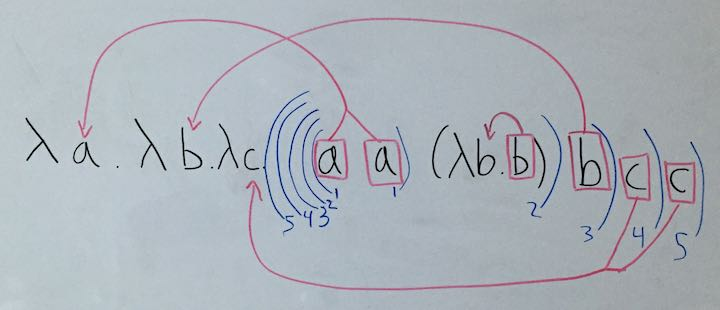
\includegraphics[scale=0.5]{i}
    \item 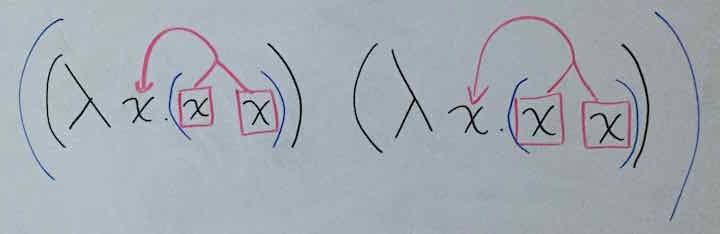
\includegraphics[scale=0.5]{ii}
    \item 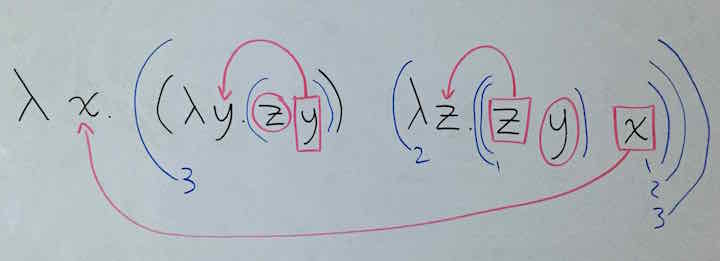
\includegraphics[scale=0.5]{iii}
  \end{enumerate}
  \item \begin{eqnarray*}
    %(\apply) \left(\left(\lambda x. \lambda z. x~z\right) (\lambda y. y)~\right{)} & \steps & b
    &        & (\apply) ~ \underline{((\lambda x. \lambda z. x~z) ~ (\lambda y. y))} \\
    & \steps & (\apply) ~ \lambda z. \underline{(\lambda y.y) ~ z} \\
    & \steps & \underline{(\apply)~\lambda z. z} \\
    & \steps & \lambda y. \underline{(\lambda z. z)~y} \\
    & \steps & \lambda y. y
  \end{eqnarray*}
\end{enumerate}
\subsection*{\sf 2 Safe Substitution}

We find counter-examples for the following rules with side conditions.

\begin{enumerate}
\item Rule : $(\lambda y . e_0) \{ e / x\} \triangleq \lambda y . (e_0 \{ e / x \})$ if $y \neq x, y \notin FV(e)$.

Let $e = y$ and $e_0 = x$ so that $y \in FV(e)$. In other word we consider the expression $\lambda y. x \{ y / x\}$.

Without the condition:

$(\lambda y. x )\{ y / x\} = \lambda y . (x \{ y / x \}) = \lambda y. y$

Under safe substitution we introduce a variable $z$:

$(\lambda y. x) \{ y / x\} = \lambda z . (x \{z / y\} \{y / x\}) = \lambda z . y$

It is easy to see that these normal forms are different as the first one is the identity function but not the second one.
\item Rule : $(\lambda y . e_0) \{ e / x\} \triangleq \lambda z . (e_0 \{z / y\}\{ e / x \})$ if $y \neq x, z \neq x, z \notin FV(e_0), z \notin FV(e)$.

Since there are 2 side conditions we will consider 2 different examples.
\begin{enumerate}
\item Let $e_0 = z$ and $e = y$ so that $z \in FV(e_0)$. The expression is $(\lambda y . z) \{ y / x \}$.

Without the condition:

$(\lambda y. z) \{ y / x\}) = \lambda z . (z \{z / y\} \{ y / x \}) = \lambda z. z$

Under safe substitution instead of $z$ we use variable $t$ so that $t \notin FV(e_0)$ and $t \notin FV(e)$

$(\lambda y. z) \{ y / x\}) = \lambda t . (z \{t / y\} \{y / x\}) = \lambda t . z$

Again these normal forms are obviously different.
\item Let $e = z \text{ } y$ and $e_0 = x$ so that $z \in FV(e)$. The expression is $(\lambda y . x) \{ z \text{ } y / x \}$.

Without the condition:

$(\lambda y . x) \{ z \text{ } y / x \}= \lambda z . (x \{z / y\} \{z \text{ } y / x \}) = \lambda z. z \text{ } y$

Under safe substitution again instead of $z$ we use variable $t$ so that $t \notin FV(e_0)$ and $t \notin FV(e)$

$(\lambda y.  x) \{ z \text{ } y / x\}) = \lambda t . (x \{t / y\} \{z \text{ } y / x\}) = \lambda t . z \text{ } y$

Again these normal forms are obviously different.
\end{enumerate}
\end{enumerate}

\subsection*{\sf 3 Small-Step Operational Semantics}
\begin{mathpar}
\Rule{Beta}{}{(\lambda x . e_0)~e_1 \steps e_0 \{ e_1 / x\}}

\Rule{MOAR POWAH}{e \steps e'}{\lambda x. e \steps \lambda x. e'}

\Rule{Step Left}{e_1 \steps e'_1}{e_1~e_2 \steps e'_1~e_2}

\Rule{Step Right}{e_2 \steps e'_2}{e_1~e_2 \steps e_1~e'_2}
\end{mathpar}

\subsection*{\sf 4 $\lambda$-Calculus Encodings}
\begin{enumerate}[(a)]
\item \verb succ $\text{ } \triangleq \lambda \widehat n f x . \text{ } f \text{ } \widehat n \text{ } (\widehat n \text{ } f \text{ } x)$

\item \verb pred $ \text{ } \triangleq \lambda \widehat n . \text{ } \widehat{n} \text{ } (\lambda x y.\text{ } x) \text{ } \widehat{0}$

\item \verb iszero $\text{ } \triangleq \lambda \widehat n . \text{ } \widehat{n} \text{ } (\lambda a b. \text{ } \verb false) \text{ } \verb true .$

\item \verb add $\text{ } \triangleq \lambda \widehat n \widehat{m}. \text{ } \widehat{n} \text{ } (\lambda a b. \text{ } \verb succ \text{ } b) \text{ } \widehat{m}.$

\verb sum $\text{ } \triangleq \lambda \widehat n . \text{ } \widehat{n} \text{ } \verb add \text{ } \widehat{0}$

\item \textbf{Karma problem: }
\end{enumerate}

\subsection*{\sf 5 $\lambda$-Calculus Programming}
Let \verb pair  be the usual pairs function that takes 2 inputs and form a pair. Let \verb p1 and \verb p2 be the usual projection operator that produces the first and second element respectively of a pair.

\verb pair $\text{ } x \text{ } y = (x,y)$

\verb p1 $\text{ } (x,y) = x$

 \verb p2 $\text{ } (x,y) = y$
\begin{enumerate}[(a)]
\item \verb curry $\text{ } \triangleq \lambda f x y. \text{ } f \text{ } (\verb pair \text{ } x \text{ } y)$

\item \verb uncurry $\text{ } \triangleq \lambda f z. \text{ } f \text{ } (\verb p1 \text{ } z) \text{ } (\verb p2 \text{ } z)$
\end{enumerate}
\subsection*{\sf 6 Implementing the $\lambda$-Calculus}
\subsection*{\sf 7 Debriefing}
\end{document}
